% Acronyms used in this chapter
\acrodef{JEPA}{Joint-Embedding Predictive Architecture}
\acrodef{EMA}{Exponential Moving Average}
\acrodef{TPE}{Tree-structured Parzen Estimator}
\acrodef{NLL}{Negative Log-Likelihood}
\acrodef{STFT}{Short-Time Fourier Transform}
\acrodef{MLP}{Multi-Layer Perceptron}

\section{Materials and Methods}

We formulate passenger movement classification as a four-class time-series task over short Wi-Fi \ac{RSSI} windows. This section details the physical collection environment, the 18-channel feature pipeline, the self-supervised world models, the supervised baselines, and the calibrated ensemble stacking framework.

\subsection{Physical Sensing Setup and Dataset Composition}

\begin{figure}[t]
\centering
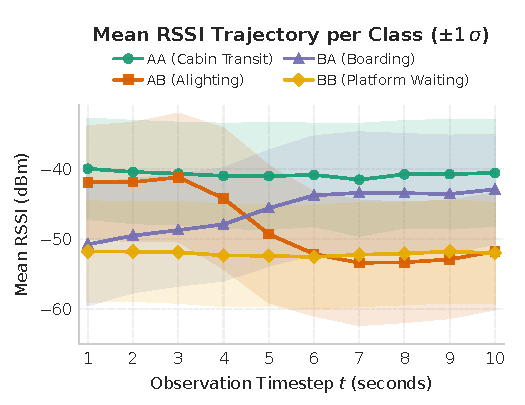
\includegraphics[width=0.72\columnwidth]{images/rssi_trajectory.pdf}
\caption{Mean RSSI trajectory per passenger movement class ($\pm 1\,\sigma$ shaded variance band) across 10-second observation windows on the 3,511-sample collection.}
\label{fig:rssi_trajectory}
\end{figure}

The physical sensing environment comprises two spatial zones relative to a municipal transit vehicle: Zone~A denotes the interior passenger cabin, and Zone~B denotes the exterior platform or bus stop. An onboard passive sniffer records 802.11 transmissions from passenger mobile devices. Spatial transitions define four mutually exclusive movement classes: internal transit (AA, Zone~A $\to$ Zone~A), alighting (AB, Zone~A $\to$ Zone~B), boarding (BA, Zone~B $\to$ Zone~A), and platform waiting (BB, Zone~B $\to$ Zone~B).

Observations consist of 10-second \ac{RSSI} sequences sampled at 1~Hz ($T=10$, $t \in \{1, \dots, 10\}$ seconds). As depicted in Figure~\ref{fig:rssi_trajectory}, each class exhibits a characteristic radio attenuation profile: internal transit (AA) maintains a high, stable signal ($\approx -40\,\text{dBm}$), alighting (AB) exhibits a monotonic decline from $-42\,\text{dBm}$ to $-52\,\text{dBm}$, boarding (BA) rises from $-51\,\text{dBm}$ to $-43\,\text{dBm}$, and platform waiting (BB) remains attenuated at $-52\,\text{dBm}$. The shaded $\pm 1\,\sigma$ variance bands capture multi-device concurrent interference while confirming the physical separability of the mobility states.

The extended dataset contains 3,511 labeled sequences, divided into 160 single-device calibration traces (pure scenario, 40 per class) and 3,351 multi-device concurrent interference traces (noise scenario, $\approx 840$ per class) collected across operational bus routes. This collection is a strict superset of the 2,251-sample collection in \cite{matos2026icaisf} under identical sensing protocols.

Data is partitioned with an 80/20 class-stratified split (seed 42), holding out 12.5\% of training data for validation ($\approx 10\%$ of total data). Training folds are augmented within folds using class-conditioned Gaussian noise ($\sigma = 0.05$) and intra-class Mixup ($\alpha = 0.4$), yielding 35,839 training samples with zero split contamination. Model selection is based on validation \ac{MCC}, and the test split is evaluated once for final reporting.

\subsection{18-Channel Rich Feature Pipeline}

To capture the temporal, statistical, and spectral dynamics of radio attenuation, we construct an 18-channel feature hierarchy from raw \ac{RSSI} $r = [r_1, \dots, r_{10}]$. The pipeline comprises four functional domains: kinematics and deviation (4 channels: raw $r_t$, velocity $\Delta_t = r_t - r_{t-1}$, acceleration $\Delta^2_t = \Delta_t - \Delta_{t-1}$, and window deviation $d_t = r_t - \mu_w$); rolling statistical moments (4 channels: rolling mean $\mu_{t,w}$, standard deviation $\sigma_{t,w}$, dynamic range $R_{t,w}$, skewness $\gamma_{t,w}$, kurtosis $\kappa_{t,w}$, and velocity sign changes); spectral descriptors (4 channels: FFT DC power $\text{band\_dc}$, AC residual energy $\text{band\_ac}$, and peak location index); and time-frequency STFT sub-bands (4 channels: Hann-windowed sub-bands $\text{stft\_b0}$ through $\text{stft\_b3}$ capturing micro-Doppler motion). The plain baseline uses only the 4 kinematic channels, whereas the rich pipeline uses all 18 channels.

\subsection{Self-Supervised World Models}

All \ac{JEPA} models learn invariant latent dynamics by predicting representations of masked or future temporal regions. An online context encoder $f_\theta$ is updated via gradient descent, a target encoder $g_\xi$ is updated via \ac{EMA} ($\xi \leftarrow \tau \xi + (1-\tau)\theta$), and a latent predictor $h_\psi$ minimizes the L2 prediction loss $\mathcal{L}_{\text{JEPA}} = \| h_\psi(f_\theta(x_c)) - \text{sg}(g_\xi(x_t)) \|_2^2$, where $\text{sg}(\cdot)$ is the stop-gradient operator. We evaluate four distinct formulations:

\textbf{T-JEPA} \cite{thimonier2024tjepa} applies per-timestep channel tokenization with learned feature embeddings and two REG tokens. Contiguous 30\% temporal masks are applied during pretraining (dim 128, 4 heads, 4 layers, width 256, 3-layer bottleneck dim 64; 0.633~M parameters, 18 channels).

\textbf{TS-JEPA} \cite{tsjepa2024} utilizes a 1D convolutional patch tokenizer (patch size two) with patch masking annealed from 0.4 to 0.7 (dim 256, 8 heads, 4 layers, width 512, 2-layer bottleneck dim 128; 2.153~M parameters, 18 channels).

\textbf{LeJEPA} \cite{balestriero2025lejepa} performs next-step autoregressive latent prediction without an \ac{EMA} target, stabilized via Sliced Gaussian Regularization (SIGReg) on the empirical characteristic function (dim 128, 4 heads, 4 layers, width 256, 3 predictor layers; 0.566~M parameters, 4 channels).

\textbf{CF-JEPA} \cite{cfjepa2026} executes mask-free multi-horizon prediction across horizons $k \in \{1, 2, 3\}$ from context crops with an \ac{EMA} target (dim 256, 8 heads, 3 layers, width 256, 1-layer bottleneck dim 128; 1.232~M parameters, 18 channels).

Pretraining runs for 300--500 epochs with AdamW, cosine annealing, gradient clipping at 1.0, and \ac{EMA} momentum schedules (0.99--0.996; 0.996--0.999 for CF-JEPA). Fine-tuning employs progressive unfreezing (frozen backbone for 25\% of epochs, then unfrozen at 0.1 learning rate with Mixup $\alpha = 0.4$ and label smoothing $\varepsilon = 0.1$).

\subsection{Supervised Classifiers and State-Space Baselines}

\textbf{SIGReg Supervised Classifier} \cite{balestriero2025lejepa} is a 3-block 1D convolutional network (192 filters) with global pooling and 128-unit projection, regularized by SIGReg ($\lambda = 0.01$) over 256 random projections (0.697~M parameters, 4 channels).

\textbf{Mamba-3 Sequence Models} \cite{gu2026mamba3} employ selective state spaces \cite{gu2023mamba} (state dim 16, rank-4 MIMO) with four front-ends: \ac{CNN} (0.945~M), \ac{TCN} \cite{bai2018tcn} (0.843~M), Transformer (0.842~M), and multi-view fusion (1.701~M) over 4 channels.

\textbf{DeepStack} is a two-stage stacked ensemble \cite{wolpert1992stacked} combining ten base models via Level-2 networks and a DeepMetaMLP (43.576~M parameters). Classical baselines include ROCKET \cite{dempster2020rocket} and catch22 \cite{lubba2019catch22}. Hyperparameters are tuned via Optuna \cite{optuna2019} with \ac{TPE} over 50 trials per model.

\subsection{Calibrated Stacking and Pareto Optimization}

Softmax logits $z_m$ from each candidate model $m$ are temperature-calibrated by optimizing scalar $T_m$ to minimize validation \ac{NLL} \cite{guo2017calibration}: $p_m = \text{softmax}(z_m / T_m)$. Calibrated probabilities are concatenated and classified via a multinomial logistic regression stacker \cite{wolpert1992stacked} with swept L2 penalties $C \in [0.005, 10.0]$. A greedy Pareto selection algorithm iteratively identifies model subsets maximizing validation \ac{MCC} per added parameter.
